\section{Gestión de clientes y contactos (desde cero)}

Los \textbf{turistas y agencias} se registran como \textbf{contactos} en Odoo. Un mismo viajero puede aparecer como \textbf{persona} (contacto individual) o, si aplica, como \textbf{empresa} (por ejemplo un operador que agrupa varios pasajeros). Para turismo receptivo, lo habitual es crear un contacto por \textbf{pasajero (PAX)} o por \textbf{grupo familiar} según cómo trabaje la agencia.

\subsection{Abrir la aplicación Contactos}

\begin{figure}[H]
    \centering
    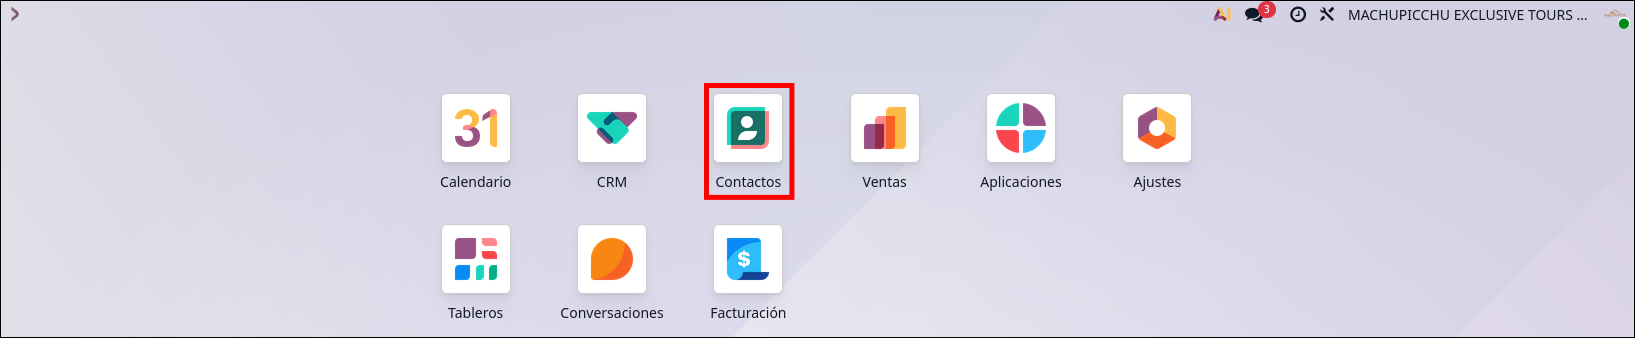
\includegraphics[width=0.95\textwidth]{assets/odoo-pantalla-principal-contactos-resaltado.png}
    \caption{Pantalla principal de Odoo: acceso a la aplicación \textbf{Contactos} (resaltada).}
\end{figure}

\begin{enumerate}
    \item En la \textbf{pantalla de aplicaciones} (icono de cuadrícula o menú principal), pulse la aplicación \textbf{Contactos}. Si no la ve, puede abrir \textbf{CRM} y desde allí usar el menú \textbf{Contactos} o la entrada equivalente que muestre su barra lateral.
    \item Se abrirá la \textbf{vista lista} de contactos con la barra superior: botón \textbf{Nuevo}, campo \textbf{Buscar...}, accesos a otras vistas (Kanban, mapa, actividad) e iconos de acción. En la tabla verá columnas como \textbf{Nombre}, \textbf{Correo electrónico}, \textbf{Teléfono}, \textbf{Actividades} y \textbf{País}.
\end{enumerate}

\begin{figure}[H]
    \centering
    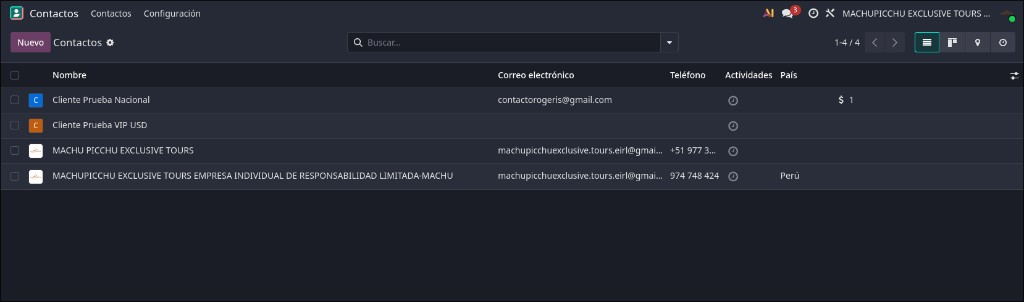
\includegraphics[width=0.98\textwidth]{assets/odoo-contactos-vista-lista-principal.png}
    \caption{Vista principal de la aplicación \textbf{Contactos} (lista). Use \textbf{Nuevo} para registrar un cliente; \textbf{Buscar...} para localizar por nombre, correo o teléfono.}
\end{figure}

\subsection{Crear un contacto nuevo}

\begin{figure}[H]
    \centering
    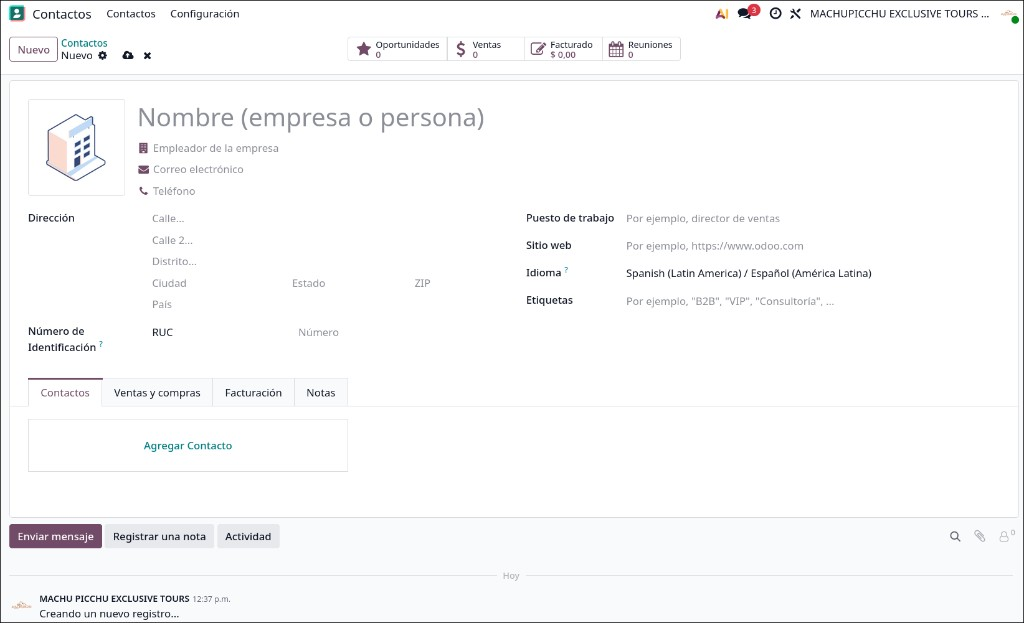
\includegraphics[width=0.95\textwidth]{assets/odoo-contactos-formulario-nuevo.png}
    \caption{Formulario que se abre al pulsar \textbf{Nuevo} en la aplicación \textbf{Contactos}.}
\end{figure}

\begin{enumerate}
    \item Pulse \textbf{Nuevo}. Se abrirá el formulario de creación del contacto (como en la imagen).
    \item Indique si el registro corresponde a una \textbf{persona} o una \textbf{empresa}:
    \begin{itemize}
        \item Para un turista individual, deje el tipo \textbf{contacto} / persona según muestre el formulario (en muchas versiones: desactivar \textbf{Es una empresa} para persona física).
        \item Para una agencia u operador, active \textbf{Es una empresa} y complete el \textbf{Nombre de la empresa}.
    \end{itemize}
    \item En el campo \textbf{Nombre} (persona) o nombre comercial, escriba el nombre tal como debe figurar en boletos y reservas cuando sea relevante.
    \item Complete al menos:
    \begin{itemize}
        \item \textbf{Correo electrónico}
        \item \textbf{Teléfono} y/o \textbf{Móvil} (el que use para WhatsApp u operador)
        \item \textbf{Dirección}: si aplica, \textbf{Ciudad}, \textbf{Provincia/Estado}, \textbf{País}
    \end{itemize}
    \item Revise la \textbf{Moneda} del contacto si el formulario la muestra: debe ser coherente con \textbf{USD} en operaciones de venta.
    \item Pulse \textbf{Guardar} (icono de nube o texto \textbf{Guardar}) para no perder los datos.
\end{enumerate}

\begin{figure}[H]
    \centering
    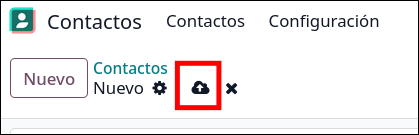
\includegraphics[width=0.95\textwidth]{assets/odoo-contactos-boton-guardar-resaltado.png}
    \caption{Formulario de contacto: botón \textbf{Guardar} resaltado para confirmar el registro.}
\end{figure}

\subsection{Buscar y editar un contacto existente}

\begin{enumerate}
    \item En la vista lista de \textbf{Contactos}, use la \textbf{búsqueda} (campo superior) escribiendo nombre, correo o teléfono.
    \item Pulse sobre la fila para abrir la \textbf{ficha del contacto}.
    \item Modifique lo necesario y pulse de nuevo \textbf{Guardar}.
\end{enumerate}

\begin{figure}[H]
    \centering
    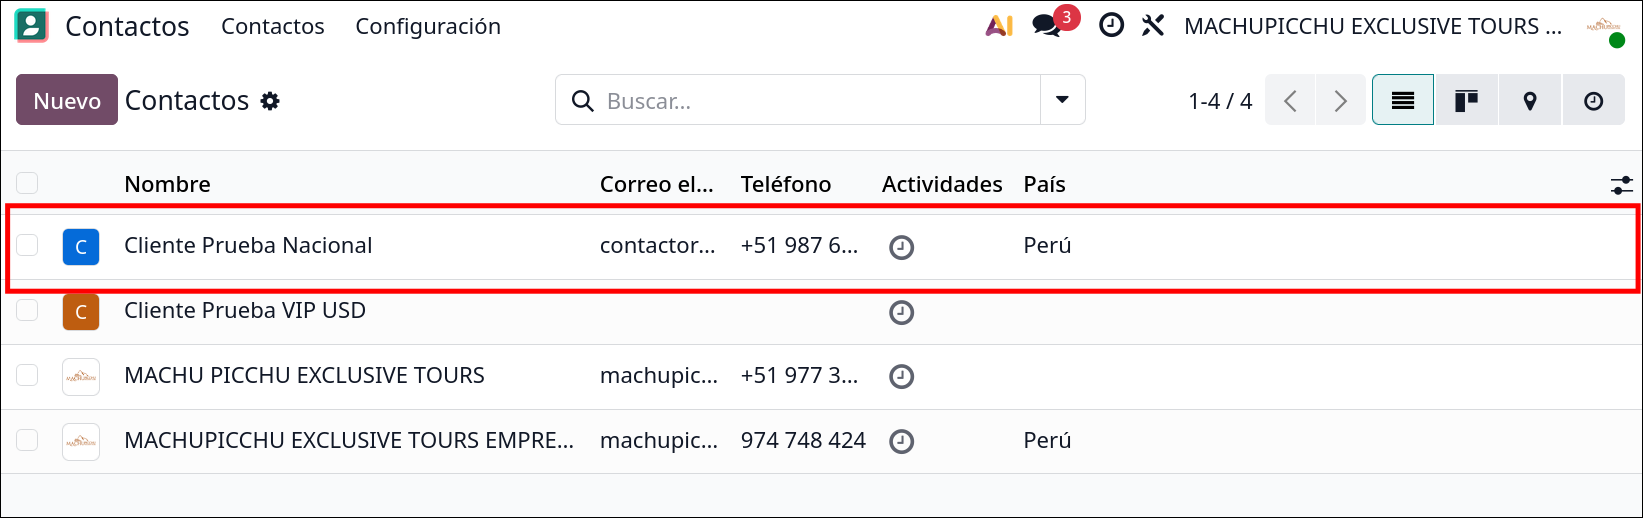
\includegraphics[width=0.95\textwidth]{assets/odoo-contactos-abrir-ficha-desde-lista.png}
    \caption{Apertura de la ficha del contacto al pulsar sobre una fila en la vista lista.}
\end{figure}

\begin{figure}[H]
    \centering
    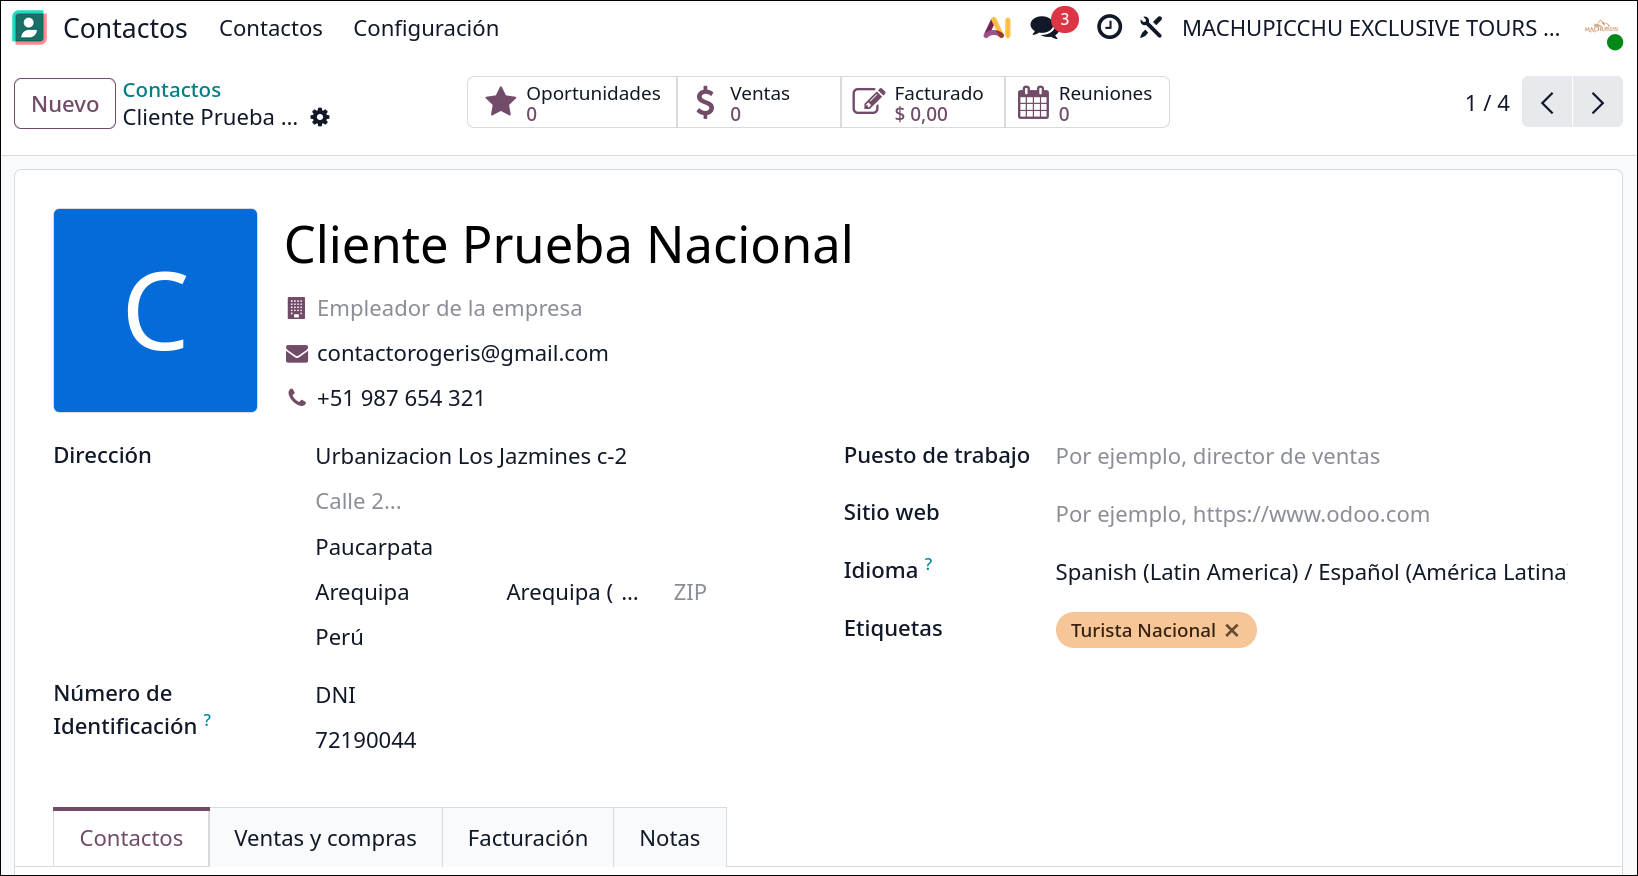
\includegraphics[width=0.95\textwidth]{assets/odoo-contactos-vista-detalle-para-editar.png}
    \caption{Vista de detalle del contacto abierta para revisar o modificar los datos y guardar los cambios.}
\end{figure}

\subsection{Ver cotizaciones, ventas y oportunidades por cliente}

\noindent\textbf{Paso 1.} Ingrese al módulo \textbf{Contactos} desde la pantalla principal de Odoo.
\begin{figure}[H]
    \centering
    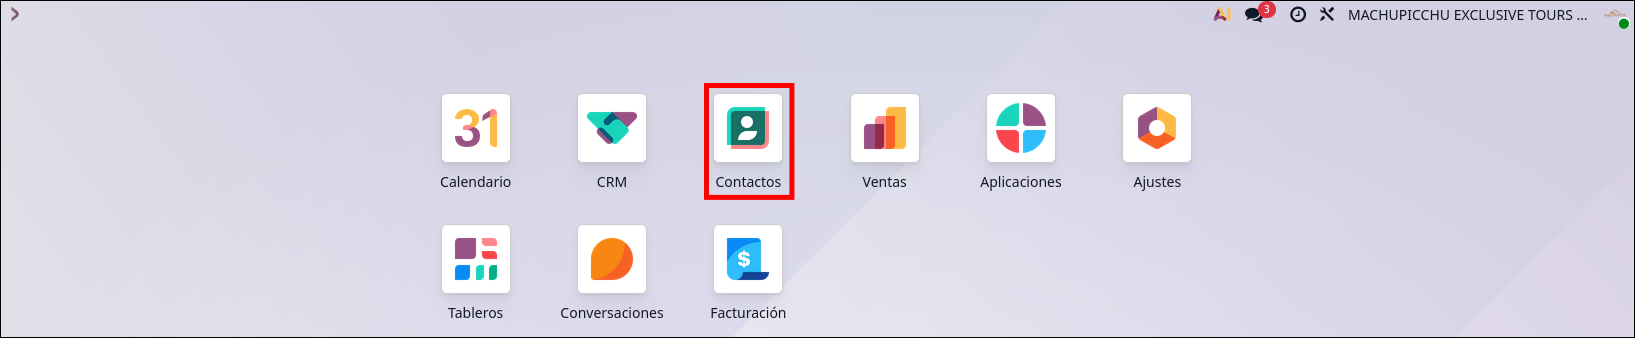
\includegraphics[width=0.95\textwidth]{assets/odoo-pantalla-principal-contactos-resaltado.png}
    \caption{Paso 1: acceso a \textbf{Contactos} desde la pantalla principal.}
\end{figure}

\noindent\textbf{Paso 2.} En la vista lista, ubique el cliente y haga clic sobre su fila para abrir su ficha.
\begin{figure}[H]
    \centering
    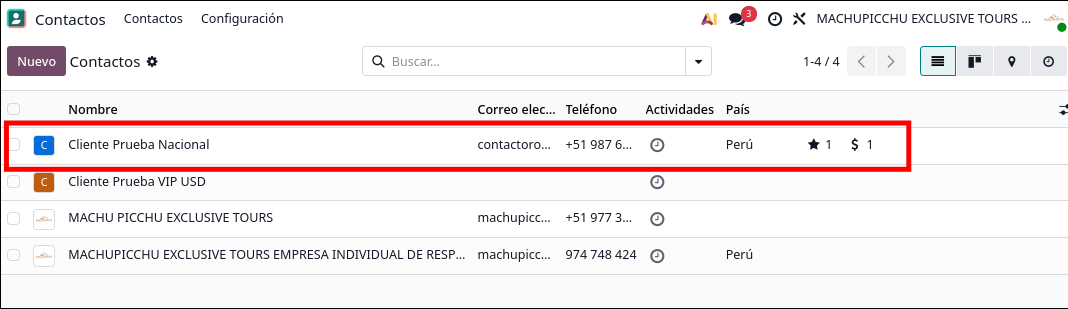
\includegraphics[width=0.95\textwidth]{assets/odoo-contactos-seleccionar-cliente-lista.png}
    \caption{Paso 2: selección del cliente desde el listado general de contactos.}
\end{figure}

\noindent\textbf{Paso 3.} Al abrir la ficha del contacto, revise el menú de indicadores (tarjetas) donde se muestran \textbf{Oportunidades}, \textbf{Ventas}, \textbf{Facturado} y \textbf{Reuniones}. Estos accesos permiten consultar rápidamente el historial comercial del cliente. Si desea ver el detalle de alguno, solo haga clic en el \textbf{cuadrito} (tarjeta) que quiera revisar.
\begin{figure}[H]
    \centering
    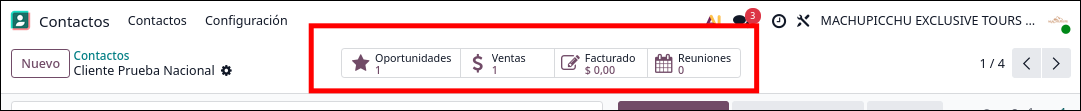
\includegraphics[width=0.95\textwidth]{assets/odoo-contactos-ficha-menu-oportunidades-ventas.png}
    \caption{Paso 3: menú de trazabilidad comercial en la ficha del contacto.}
\end{figure}

\subsection{Pestañas y chatter útiles}

Según los módulos instalados, en la ficha puede ver pestañas como:

\begin{itemize}
    \item \textbf{Notas internas}: observaciones solo para el equipo (no suelen salir al cliente en PDF salvo que usted las use en otro flujo).
    \item \textbf{Ventas y compras}: condiciones de pago, lista de precios, si estuvieran asignadas.
    \item Zona derecha o inferior: \textbf{chatter} (mensajes, registro de actividades, seguidores). Use \textbf{Enviar mensaje} para dejar notas internas con menciones si su equipo lo usa.
\end{itemize}

\begin{figure}[H]
    \centering
    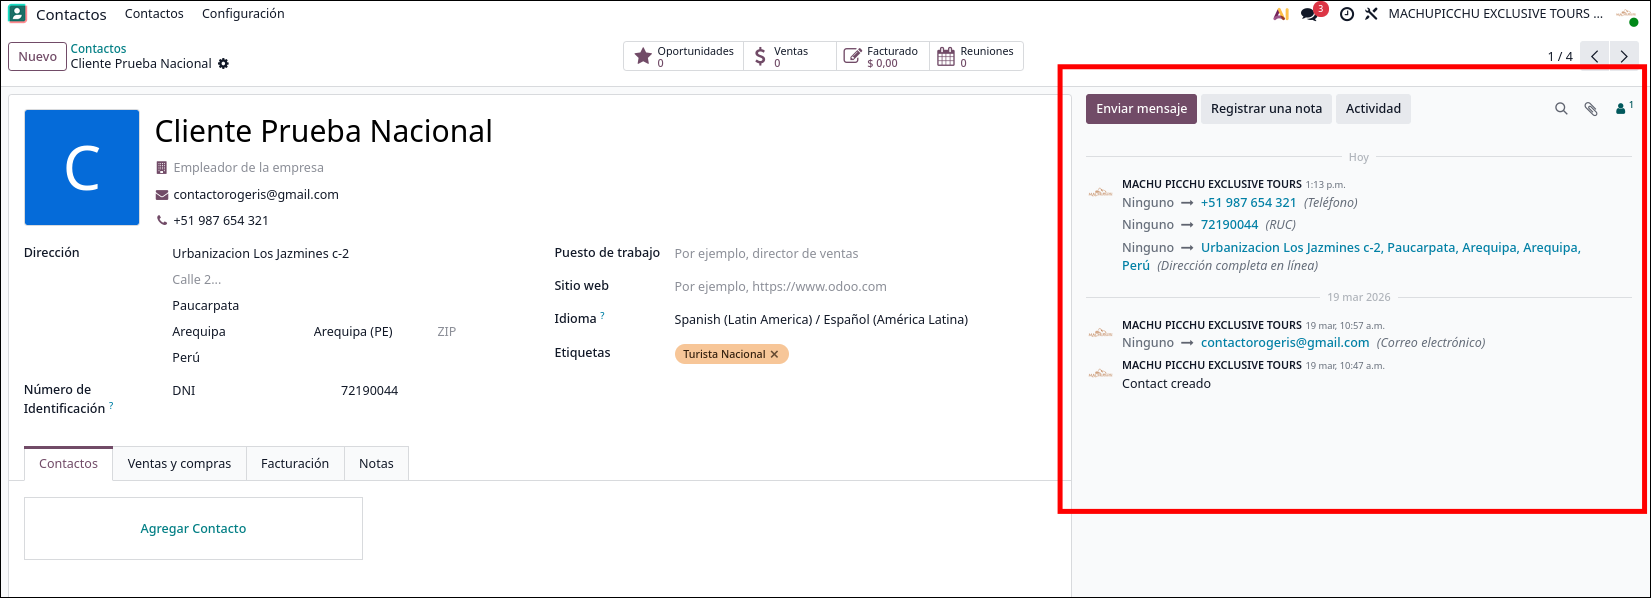
\includegraphics[width=0.95\textwidth]{assets/odoo-contactos-pestanas-y-chatter-resaltado.png}
    \caption{Pestañas de la ficha y zona de \textbf{chatter} resaltadas para identificar dónde revisar y registrar seguimiento interno.}
\end{figure}

\subsection{Adjuntar documentos (pasaporte u identificación)}

Para compra de ingresos y controles con nombre exacto:

\begin{enumerate}
    \item Abra la ficha del contacto guardada.
    \item En el \textbf{chatter} o zona de \textbf{adjuntos} (según la vista: icono de clip, \textbf{Adjuntos} o arrastrar archivo), cargue una \textbf{foto o PDF legible} del pasaporte o documento.
    \item No sustituya el archivo por mensajes de WhatsApp fuera del sistema: mantenga la copia en la ficha como respaldo institucional.
\end{enumerate}

\begin{figure}[H]
    \centering
    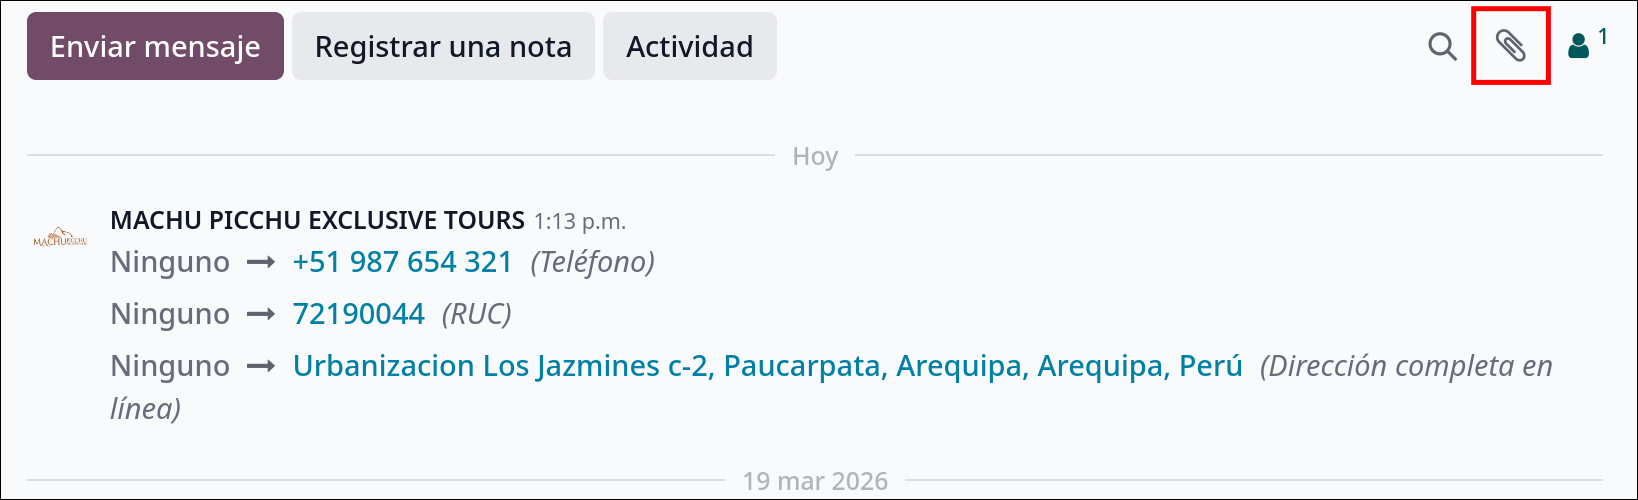
\includegraphics[width=0.95\textwidth]{assets/odoo-contactos-adjuntar-documento-clip-resaltado.png}
    \caption{Zona de adjuntos con el icono de clip resaltado para cargar pasaporte o documento en la ficha del contacto.}
\end{figure}

\begin{figure}[H]
    \centering
    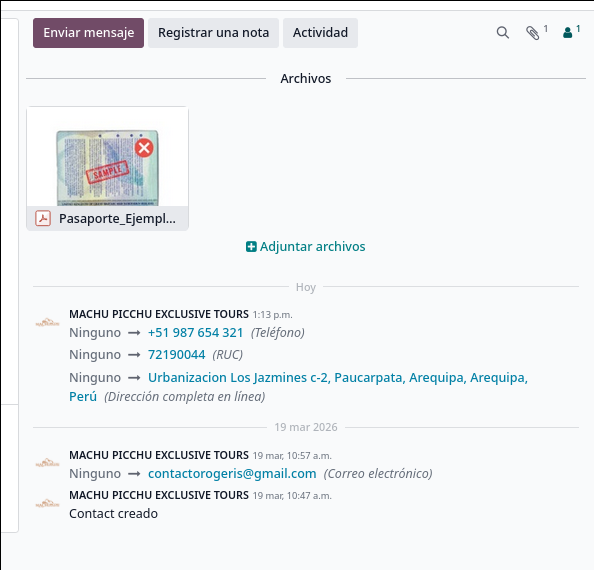
\includegraphics[width=0.95\textwidth]{assets/odoo-contactos-pasaporte-adjunto-ejemplo.png}
    \caption{Ejemplo de pasaporte adjunto en la ficha del contacto para respaldo documental.}
\end{figure}

\subsection{Datos mínimos que debe capturar para cada cliente (PAX o contacto operativo)}

Registre \textbf{solo lo necesario} para vender, cobrar y emitir/comprar servicios sin errores. Lista de referencia para \textbf{Machu Picchu Exclusive Tours}:

\begin{itemize}
    \item \textbf{Nombre completo} (como en documento de viaje / pasaporte cuando deba coincidir con tren o ingreso).
    \item \textbf{Correo electrónico} (canal formal de cotización y confirmaciones).
    \item \textbf{Teléfono o móvil} (incluido prefijo internacional; el que use para coordinación).
    \item \textbf{País} (y ciudad si ayuda al segmento o envío de información).
    \item \textbf{Idioma de atención} si lo anota en notas o campo disponible (español, inglés, portugués, etc.).
    \item \textbf{Número de documento} (pasaporte o DNI) cuando ya lo tenga y deba quedar registrado para compras; si no, al menos el \textbf{adjunto} del documento escaneado o foto.
    \item \textbf{Fecha de nacimiento} solo si un proveedor o ingreso la exige para el servicio.
    \item \textbf{Restricciones alimentarias o médicas relevantes} solo si afectan el servicio (opcional, suele ir en \textbf{Notas internas}).
    \item \textbf{Adjunto}: imagen/PDF de pasaporte o ID cuando entre en etapa de compra de tickets no modificables.
\end{itemize}

\noindent\textbf{No es obligatorio} llenar campos vacíos que no use la operación (por ejemplo datos fiscales complejos) salvo que su contador o proceso local los requiera más adelante.

\subsection{Relación con el CRM (siguiente capítulo)}

Una vez existe el \textbf{contacto}, podrá vincularlo a una \textbf{oportunidad} en el CRM (embudo de ventas). El contacto es la \textbf{ficha maestra} del cliente; la oportunidad es el \textbf{trato en curso} (presupuesto, negociación, ganado).
